\documentclass[handout,nooutcomes,noauthor]{ximera}

\graphicspath{  
{./}
{./whoAreYou/}
{./drawingWithTheTurtle/}
{./bisectionMethod/}
{./circles/}
{./anglesAndRightTriangles/}
{./lawOfSines/}
{./lawOfCosines/}
{./plotter/}
{./staircases/}
{./pitch/}
{./qualityControl/}
{./symmetry/}
{./nGonBlock/}
}


%% page layout
\usepackage[cm,headings]{fullpage}
\raggedright
\setlength\headheight{13.6pt}


%% fonts
\usepackage{euler}

\usepackage{FiraMono}
\renewcommand\familydefault{\ttdefault} 
\usepackage[defaultmathsizes]{mathastext}
\usepackage[htt]{hyphenat}

\usepackage[T1]{fontenc}
\usepackage[scaled=1]{FiraSans}

%\usepackage{wedn}
\usepackage{pbsi} %% Answer font


\usepackage{cancel} %% strike through in pitch/pitch.tex


%% \usepackage{ulem} %% 
%% \renewcommand{\ULthickness}{2pt}% changes underline thickness

\tikzset{>=stealth}

\usepackage{adjustbox}

\setcounter{titlenumber}{-1}

%% journal style
\makeatletter
\newcommand\journalstyle{%
  \def\activitystyle{activity-chapter}
  \def\maketitle{%
    \addtocounter{titlenumber}{1}%
                {\flushleft\small\sffamily\bfseries\@pretitle\par\vspace{-1.5em}}%
                {\flushleft\LARGE\sffamily\bfseries\thetitlenumber\hspace{1em}\@title \par }%
                {\vskip .6em\noindent\textit\theabstract\setcounter{question}{0}\setcounter{sectiontitlenumber}{0}}%
                    \par\vspace{2em}
                    \phantomsection\addcontentsline{toc}{section}{\thetitlenumber\hspace{1em}\textbf{\@title}}%
                     }}
\makeatother



%% thm like environments
\let\question\relax
\let\endquestion\relax

\newtheoremstyle{QuestionStyle}{\topsep}{\topsep}%%% space between body and thm
		{}                      %%% Thm body font
		{}                              %%% Indent amount (empty = no indent)
		{\bfseries}            %%% Thm head font
		{)}                              %%% Punctuation after thm head
		{ }                           %%% Space after thm head
		{\thmnumber{#2}\thmnote{ \bfseries(#3)}}%%% Thm head spec
\theoremstyle{QuestionStyle}
\newtheorem{question}{}



\let\freeResponse\relax
\let\endfreeResponse\relax

%% \newtheoremstyle{ResponseStyle}{\topsep}{\topsep}%%% space between body and thm
%% 		{\wedn\bfseries}                      %%% Thm body font
%% 		{}                              %%% Indent amount (empty = no indent)
%% 		{\wedn\bfseries}            %%% Thm head font
%% 		{}                              %%% Punctuation after thm head
%% 		{3ex}                           %%% Space after thm head
%% 		{\underline{\underline{\thmname{#1}}}}%%% Thm head spec
%% \theoremstyle{ResponseStyle}

\usepackage[tikz]{mdframed}
\mdfdefinestyle{ResponseStyle}{leftmargin=1cm,linecolor=black,roundcorner=5pt,
, font=\bsifamily,}%font=\wedn\bfseries\upshape,}


\ifhandout
\NewEnviron{freeResponse}{}
\else
%\newtheorem{freeResponse}{Response:}
\newenvironment{freeResponse}{\begin{mdframed}[style=ResponseStyle]}{\end{mdframed}}
\fi



%% attempting to automate outcomes.

%% \newwrite\outcomefile
%%   \immediate\openout\outcomefile=\jobname.oc
%% \renewcommand{\outcome}[1]{\edef\theoutcomes{\theoutcomes #1~}%
%% \immediate\write\outcomefile{\unexpanded{\outcome}{#1}}}

%% \newcommand{\outcomelist}{\begin{itemize}\theoutcomes\end{itemize}}

%% \NewEnviron{listOutcomes}{\small\sffamily
%% After answering the following questions, students should be able to:
%% \begin{itemize}
%% \BODY
%% \end{itemize}
%% }
\usepackage[tikz]{mdframed}
\mdfdefinestyle{OutcomeStyle}{leftmargin=2cm,rightmargin=2cm,linecolor=black,roundcorner=5pt,
, font=\small\sffamily,}%font=\wedn\bfseries\upshape,}
\newenvironment{listOutcomes}{\begin{mdframed}[style=OutcomeStyle]After answering the following questions, students should be able to:\begin{itemize}}{\end{itemize}\end{mdframed}}



%% my commands

\newcommand{\snap}{{\bfseries\itshape\textsf{Snap!}}}
\newcommand{\flavor}{\link[\snap]{https://snap.berkeley.edu/}}
\newcommand{\mooculus}{\textsf{\textbf{MOOC}\textnormal{\textsf{ULUS}}}}


\usepackage{tkz-euclide}
\tikzstyle geometryDiagrams=[rounded corners=.5pt,ultra thick,color=black]
\colorlet{penColor}{black} % Color of a curve in a plot



\ifhandout\newcommand{\mynewpage}{\newpage}\else\newcommand{\mynewpage}{}\fi

\title{Area of triangles}

\author{Jenny Sheldon \and Bart Snapp}

\begin{document}
\begin{abstract}
  Derive the formula for the area of a triangle!
\end{abstract}
\maketitle


\begin{listOutcomes}
\item Give the standard formula for the area of a triangle.
\item Explain Cavalieri's principle.
\item Explain why the formula for the area of a triangle is true.
\item Explain how shapes of the same area can have a arbitrarily large
  perimeters.
\end{listOutcomes}


\mynewpage



\begin{question} 
  Explain how the following picture ``proves'' that the area of a RIGHT
  triangle is one half of the base times the height.
  \begin{center}
  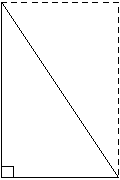
\includegraphics{pbpAreaRight.pdf}
  \end{center}
  \begin{freeResponse}
    We know that the area of a rectangle of height $h$ and width $b$
    has area $h\cdot b$. However, we can also see that every right
    triangle can be placed in such a rectangle, while occupying
    exactly half the area. Hence the area of a RIGHT triangle is:
    \[
    \text{Area of right triangle} = \frac{bh}{2}
    \]
  \end{freeResponse}
\end{question}
\mynewpage


\begin{question}
  ``Shearing'' is a process where you take a shape, cut it into thin strips, 
  then push the strips around in one direction to make a new shape.  
  Cavalieri's principle states:\index{Cavalieri's principle}
  \begin{quote}
    Shearing parallel to a fixed direction does not change the
    $n$-dimensional measure of an object.
  \end{quote}
  EXPLAIN how the first problem, combined with the following
  picture ``proves'' (via Cavalieri's principle) that the area of ANY
  triangle is one half of the base times the height.
  \begin{center}
  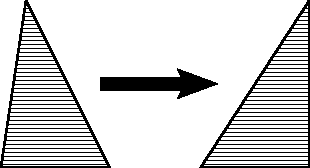
\includegraphics{pbpShearTri.pdf}
  \end{center}
  \begin{freeResponse}
    If we want to know the area of any triangle, simply shear it to be a right triangle:
    \[
    \text{MISSING PICTURE}
    \]
    Since shearing doesn't change the area, by Cavalieri's principle,
    we see this right triangle has the same area as our original
    triangle. Thus the area of the original triangle is:
    \[
    \text{Area of any triangle} = \frac{bh}{2}
    \]
  \end{freeResponse}
\end{question}
\mynewpage


\begin{question} Finally:
  \begin{enumerate}
  \item Give an intuitive argument explaining why Cavalieri's
    principle is true.
  \item Explain how to use a picture to ``prove'' that a triangle of a
    given (fixed) area could have an ARBITRARILY LARGE perimeter.
  \end{enumerate}
  \begin{freeResponse}
    \begin{enumerate}
    \item Imagine our triangle as being a cross section of stacked
      papers. Moving these papers around doesn't change the area of
      each of the slices, hence, shearing doesn't change the area.
    \item Consider this picture:
      \[
      \text{MISSING PICTURE}
      \]
      From this we can make a triangle with an arbitrarily large
      perimeter with a fixed area.
    \end{enumerate}
  \end{freeResponse}
\end{question}

\end{document}
